\documentclass[usenatbib]{mn2e} 
\usepackage{amsmath} 
\usepackage{amssymb} 
\usepackage{graphics}
\usepackage{graphicx}
\usepackage{epsfig} 
\usepackage{float} 
\def\be{\begin{equation}}
\def\ee{\end{equation}}
\def\ba{\begin{eqnarray}}
\def\ea{\end{eqnarray}}

% To highlight comments 
\usepackage{color}
\definecolor{red}{rgb}{1,0.0,0.0}
\newcommand{\red}{\color{red}}
\definecolor{blue}{rgb}{0.1,0.3,0.9}
\newcommand{\blue}{\color{blue}}

\usepackage[normalem]{ulem}
\definecolor{darkgreen}{rgb}{0.0,0.5,0.0}
\newcommand{\SRK}[1]{\textcolor{darkgreen}{\bf SRK: \textit{#1}}}
\newcommand{\SRKED}[1]{\textcolor{darkgreen}{\bf #1}}

\newcommand{\LCDM}{$\Lambda$CDM~}
\newcommand{\beq}{\begin{eqnarray}}  
\newcommand{\eeq}{\end{eqnarray}}  
\newcommand{\zz}{$z\sim 3$} 
\newcommand{\apj}{ApJ}  
\newcommand{\apjs}{ApJS}  
\newcommand{\apjl}{ApJL}  
\newcommand{\aj}{AJ}  
\newcommand{\mnras}{MNRAS}  
\newcommand{\mnrassub}{MNRAS accepted}  
\newcommand{\aap}{A\&A}  
\newcommand{\aaps}{A\&AS}  
\newcommand{\araa}{ARA\&A}  
\newcommand{\nat}{Nature}  
\newcommand{\physrep}{PhR}
\newcommand{\pasp}{PASP}    
\newcommand{\pasj}{PASJ}    
\newcommand{\avg}[1]{\langle{#1}\rangle}  
\newcommand{\ly}{{\ifmmode{{\rm Ly}\alpha}\else{Ly$\alpha$}\fi}}
\newcommand{\hMpc}{{\ifmmode{h^{-1}{\rm Mpc}}\else{$h^{-1}$Mpc }\fi}}  
\newcommand{\hGpc}{{\ifmmode{h^{-1}{\rm Gpc}}\else{$h^{-1}$Gpc }\fi}}  
\newcommand{\hmpc}{{\ifmmode{h^{-1}{\rm Mpc}}\else{$h^{-1}$Mpc }\fi}}  
\newcommand{\hkpc}{{\ifmmode{h^{-1}{\rm kpc}}\else{$h^{-1}$kpc }\fi}}  
\newcommand{\hMsun}{{\ifmmode{h^{-1}{\rm {M_{\odot}}}}\else{$h^{-1}{\rm{M_{\odot}}}$}\fi}}  
\newcommand{\hmsun}{{\ifmmode{h^{-1}{\rm {M_{\odot}}}}\else{$h^{-1}{\rm{M_{\odot}}}$}\fi}}  
\newcommand{\Msun}{{\ifmmode{{\rm {M_{\odot}}}}\else{${\rm{M_{\odot}}}$}\fi}}  
\newcommand{\msun}{{\ifmmode{{\rm {M_{\odot}}}}\else{${\rm{M_{\odot}}}$}\fi}}  
\newcommand{\lya}{{Lyman$\alpha$~}}
\newcommand{\clara}{{\texttt{CLARA}}~}
\newcommand{\rand}{{\ifmmode{{\mathcal{R}}}\else{${\mathcal{R}}$ }\fi}}  
\newcommand{\hs}{{\hspace{1mm}}}  
\newcommand{\kms}{\,km~s$^{-1}$}

% definition to produce a "less than or similar to" symbol
\def\lsim{~\rlap{$<$}{\lower 1.0ex\hbox{$\sim$}}}

% definition to produce a "greater than or similar to" symbol
\def\gsim{~\rlap{$>$}{\lower 1.0ex\hbox{$\sim$}}}

\begin{document}

\title[Rotation in the Lyman-$\alpha$ line]{Effects of rotation on the
  Lyman-$\alpha$ line morphology in distant galaxies}
\author[N. Garavito and J.E. Forero-Romero]{
\parbox[t]{\textwidth}{\raggedright 
  Nicolas Garavito-Camargo.$^{1}$ 
  Jaime E. Forero-Romero$^{2}$ 
}
\vspace*{6pt}\\
$^{1}$Universidad de los Andes
$^{2}$Uni B
}
\maketitle

\begin{abstract}
Rotation is present in the gas kinematics of galaxies up to the
highest redshifts. In this paper we present for the first time
radiative transfer calculations that show the impact of rotation on
the morphology of the Lyman $\alpha$ line. To this end we construct
simplified models where a galaxy is modeled as an homogeneous sphere
composed as an homogenous mixture of dust and hydrogen at a constant
temperature. These spheres have an solid-body rotation with linear
velocities at the surface in the range $0-300$ \kms. We consider
radiation sources both in the center of the rotating cloud and also
homogeneously distributed around the sphere. We find that higher
rotational velocities increase the width of each peak in the outgoing
line profile while it also increases the amount of Lyman alpha photons
escaping in the line center. This trends makes that for high
rotational velocities and large Hydrogen optical depths the double
peak of the line tends to be erased an be replaced by a single peak the
lines center. This is more pronounced for radiation sources
homogeneously distributed. Concerning the escape fraction we find that
rotation does not have any effect, provided that all the sources are
centrally emitted. However in the case of homogeneously emitted
sources we measure an increase of about a factor of $2$ in the escape
fraction for higher rotational velocity vealues.


Our work shows clearly that gas rotation has a non
negligeable impact on the shape of the Lyman $\alpha$ line.

\end{abstract}
\begin{keywords}
galaxies: high-redshift - galaxies: star formation - line: formation
\end{keywords}


\section{Introduction}
\label{sec:intro}

Due to the resonant nature of the lyman alpha line, gas kinematics
play an important role shaping its morphology. In the literature there
has been extensive studies of outflow/inflow configurations. 

In this paper we study for the first time the impact of rotation on
the morphology of the Lyman $\alpha$ line. To isolate the effects of
rotation we focus on a simple system: the gas distribution is
spherical, with homogenous density and the gas rotates as a solid
body.

This paper is paper is structured as follows.



\section{Implementation of Bulk Gas Rotation}
\label{sec:implementation}

We implement into CLARA the simplest model whereby a sphere rotates
with homogeneous angular velocity. We define a cartesian coordinate
system with its origin at the center of the sphere and the rotation
axis to be the $z$-axis, the components in the bulk velocity field, $\vec{v}
= v_{x}\hat{i} + v_{y}\hat{j} + v_{z}\hat{k}$. in the gas can be written as 
 
\begin{subequations}
\begin{align}
    v_{x}=-\dfrac{y}{R}V_{\rm max}, \label{subeq1}\\
    v_{y}=\dfrac{x}{R}V_{\rm max}, \label{subeq2}\\
    v_{z}=0, \label{subeq3}
\end{align}
\end{subequations}

where $R$ is the radius of the sphere and $V_{\rm max}$ is the linear
velocity at the sphere's surface. The minus sign in the x-component of
the velocity indicates the direction of rotation, in this case we
assume that the angular velocity vector goes in the $\hat{k}$
direction.  The linear dependence of the velocity on the radial
distance describes the case of constant angular velocity
$\omega=V_{\rm max}/R$.  

We take the polar angle $\theta$ that a unitary vector makes with the
rotation axis as defined by the dot product $\cos\theta =
{\hat{u}\cdot\hat{k}}$. In the Section \ref{sec:results} we will
present in detail how the line differs at different observing angles
$\theta$. 



\section{Grid of Simulated Models}
\label{sec:models}

We compute the emergent Lyman-$\alpha$ line for several models with
differents values for the maximal rotational velocity, hydrogend optical
depth, dust optical depth and initial distributions of the photons
with respect to the gas. There are in total 60 models with the input
parameters summarized in Table  \ref{table:models}. 

\begin{table}
\begin{center}
\begin{tabular}{ccc}\hline
Velocity (\kms) & $V_{\rm max}$&$0,\ 50,\ 100,\ 200,\ 300$\\
Hydrogen Optical Depth & $\tau_{H} $ & $10^{5},\ 10^{6},\ 10^{7}$\\
Dust Optical Depth & $\tau_{A}$ & $0$,$1$\\
Photons Distributions & & Central, Homogeneous\\
\hline
\end{tabular}
\caption{
Values for the varying input parameters in CLARA. Taking into account
all the possible combinations for these models
} 
\label{table:models}
\end{center}
\end{table}




%poner las graficas para un modelo dado poner el efecto de
%la rotación (poner %uno con velocidad cero) y del observador. 



\section{Results}
\label{sec:results}

The central result of this paper is summarized in
Fig.~\ref{fig:DifferentVelocities} where we show that rotation has a
considerable effect on the morphology of the emergent Lyman-alpha line
both in the case where the photons are emitted at the sphere's center
and when they are initialized with an homogeneous distribution all
over the gas volume.

The results for these outgoing spectra are integrated over the whole
sphere, meaning that all the escaping photons were taking into account
regardless of the direction of the outgoing photons. Figure
\ref{fig:DifferentObservers} shows how if one gives a weight to each outgoing
photon according to its direction when escaping the gas distribution
it is posible to detect notable differences in the spectrum for
different viewing angles.



\begin{figure*}
  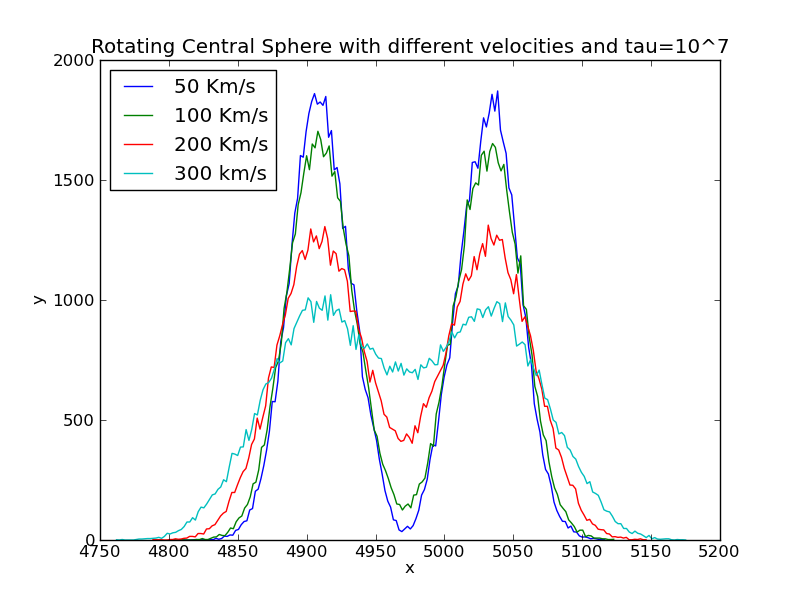
\includegraphics[width=0.45\textwidth]{7tDifSpeedsZ.png}
  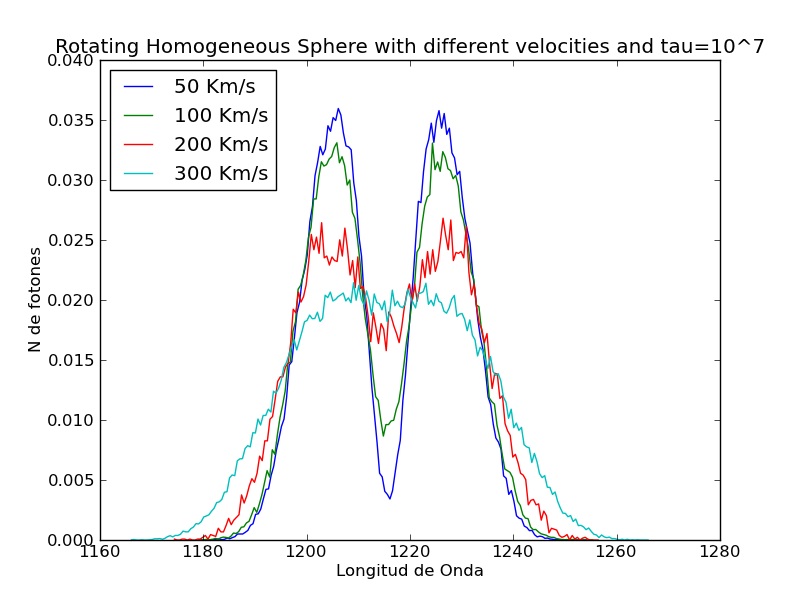
\includegraphics[width=0.45\textwidth]{7tHOMDifSpeeds1.png}
\caption{Shape of the lyman alpha line for
    differents velocities. The left (right) panel shows the central
    (homogeneous) photon distribution. All photons were taken into
    account regardless of their outgoing direction of propagation.
  \label{fig:differentvelocities}}
\end{figure*}

\begin{figure*}
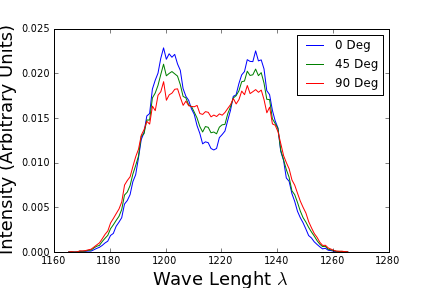
\includegraphics[width=0.45\textwidth]{Observers7t.png}
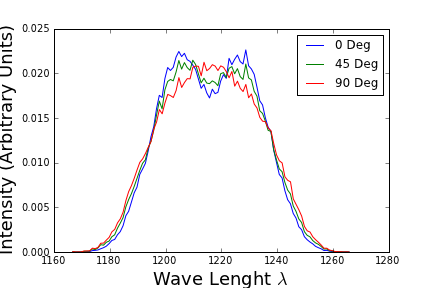
\includegraphics[width=0.45\textwidth]{Observers7tHOM.png}
\caption{Same as Figure \ref{fig:differentvelocities} but this time
  the differen lines show the line morphology for different polar angles
  $\theta$ with respect to the rotation axis. In this case each photon
  has a weight dependent on their outgoing direction. All spectra correspond
  to the same $V_{\rm max}=300$\kms, Optical   Depth $\tau=10^{7}$ and
  Central Distribution without dust.}  
  \label{fig:differentobservers}
\end{figure*}


In the following subsections we quantify the trends observed in
Fig. \ref{fig:differentvelocities} and
Fig. \ref{fig:differentobservers} as a function of the maximum
rotation velocity $V_{\rm max}$ and the position of the observer with
respect to the rotation angle, $\mu = \cos{\theta}$. All the results
in this section will be expressed in terms of resframe wavelength.

First we quantify the line by its full width at half maximum
(FWHM) and the peak positions. In order to interpret these results we
measure how the rotation affects the average number of scatterings
for each Lyman-alpha photon in the simulation. This help us to
introduce the next subsection on the escape fraction in our models
including dust. We conclude the section by estimating the
expected line flux for top hat filters at a fixed center and varying
width. 

\subsection{Line width and peak maxima}
\label{sec:widthpeak}


\begin{figure*}
    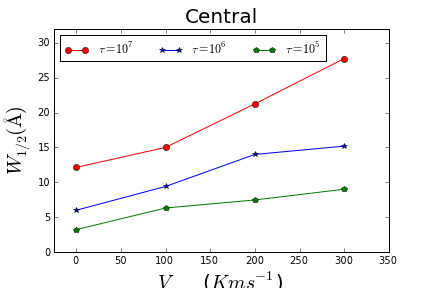
\includegraphics[width=0.45\textwidth]{WidthCentral.png}
    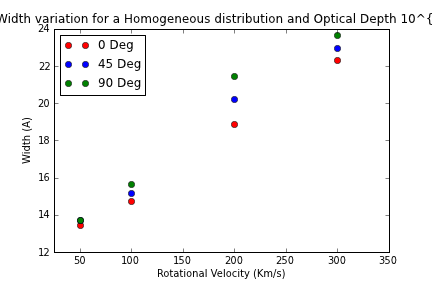
\includegraphics[width=0.45\textwidth]{WidthHomogeneous.png}
   \caption{Width of the lyman-alpha line for all the models.   \label{fig:widthvsvelocity}}
\end{figure*}


\begin{figure*}
    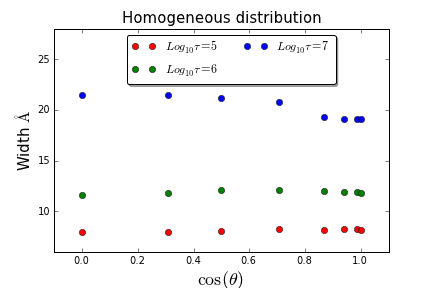
\includegraphics[width=0.45\textwidth]{WidthvsThetaDifODHOM.png}
    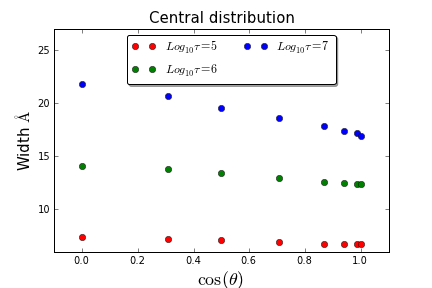
\includegraphics[width=0.45\textwidth]{WidthvsThetaDifOD.png}
    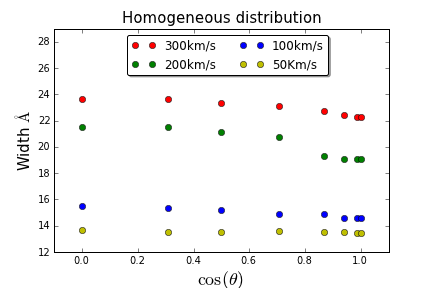
\includegraphics[width=0.45\textwidth]{WidthvsThetaDifSpeedsHOM.png}
    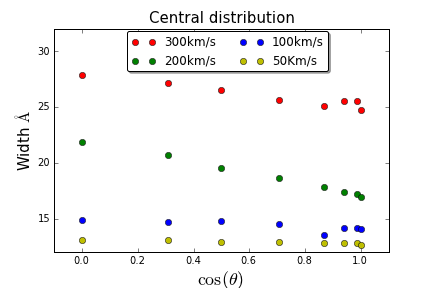
\includegraphics[width=0.45\textwidth]{WidthvsThetaDifSpeeds.png}
\caption{Width of the lyman-alpha line for all the models. 
  \label{figure:widthvstheta}
}
\end{figure*}

The first quantitative conclusion of the effect of rotation in the
Lyman alpha line is that the double peaks in the line tend to broaden
until they reach a single broad emission peak. This is most evident in
the case of Lyman-alpha sources homogeneously distributed in the gas
distributions (Fig. \ref{differentvelocities} right panel).

To quantify the line broadening we measure a modified version of the full
width at half maximum (FWHM) for half of the line, $W_{1/2}$. It means that in
the case of double peaked emission, $W_{1/2}$ corresponds to the with
one of thepeaks, while in the extreme case when the line is converted
into a single peak, $W_{1/2}$ corresponds to half of the full width. 

This definition allows us to quantify the line width both in the cases
of double and single peak emission. Furthermore it has the advantage
that this line width should have a direct observational correspondence
to the observed line feature once the Inter-Galactic Medium (IGM)
effects are taken into account, which have the central effect of
strongly reducing the intensity of the blue peak of the line.

Figure~\ref{fig:widthvsvelocity} summarizes our findings for $W_{1/2}$
as a function of $V_{\rm max}$. The line width increases with the
rotational velocity of the gas cloud. This increase can be of a factor
of $2-3$ with respect to the width with respect to the static
case. This trend is conserved at all optical depths regardless of the
initial source distribution. 

This result includes all the outgoing photons, regardless of the
position of the observer. In Figure~\ref{fig:widthvstheta} we
take into account the different positions of the observer in the
measurement of the half-width $W_{1/2}$. From this we conclude
that observers with a line of sight perpendicular to the axis of
rotation (i.e. edge-on in the case of spiral galaxy) tend to meaure
larger line widths than observers aligned with the rotation axis
(i.e. face-on). The influence of the observer position on the line
width, amounting always less than $15\%$ of a difference with respect
to the result that takes into account all the outgoing photons with
the same weight regardless of the relative observer position.

%Both for central and homogeneous distribution of sources, We found a
%dependency of the width with the rotation velocity of the gas cloud,
%this results are summarize in Figure ~\ref{figure:width}. As velocity
%increase also the equivalent width increase (for both homogeneous and
%central distribution), it means that some photons escape with fewer
%scatterings than the static case but at the same time a few photons escape with% more scatterings, this can be seen clearly in
%Figure. (Nscatt)\\ 

%We also found a dependency with the viewing angles, in particular as
%the angle increase the width also increase Figure
%~\ref{fig:withvstheta}, this was also found in Verhemme et al. 2012
%for a rotating disk but the pure effect of rotation can not been study
%as it is in our case. Following the convention of Verhamme et al 2012
%we define $\mu=cos(\theta)$, and we can make a polynomial fit for the
%$FWHM(\mu)$ for our models, this is resumed in Table ~\ref{table:fits} 


\begin{figure*}
    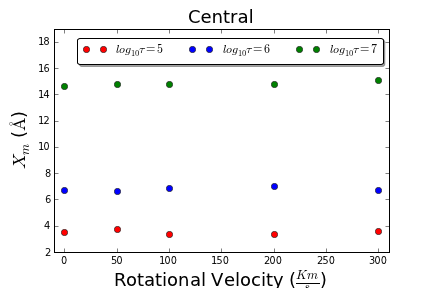
\includegraphics[width=0.45\textwidth]{maximumvsvelocitiesDifODCentral.png}
    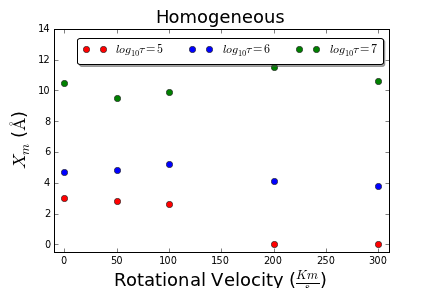
\includegraphics[width=0.45\textwidth]{maximumvsvelocitiesDifODHOM.png}
\caption{Position of the maxima
    in the outgoing spectra for differents Rotational velocities,
    (up)Central Distriution, (Down) Homogeneous Distribution.\label{fig:maximumsvsvelocity}} 
\end{figure*}

\begin{figure*}
    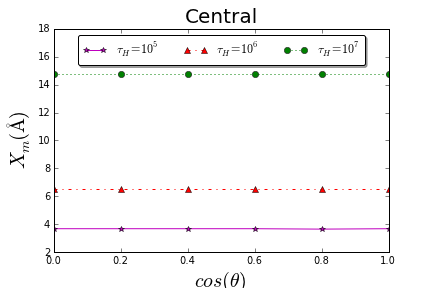
\includegraphics[width=0.45\textwidth]{maximumvscosthetaHOMSameSpeed.png}
    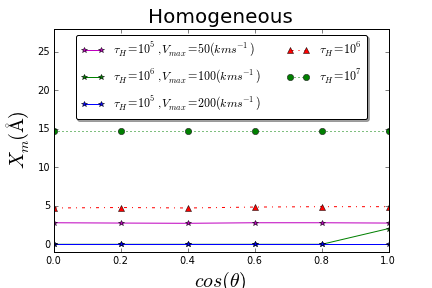
\includegraphics[width=0.45\textwidth]{maximumvscosthetaDifSpeedCentral.png}
\caption{Position of the maxima
    in the outgoing spectra for differents Rotational velocities,
    (up)Central Distriution, (Down) Homogeneous Distribution.\label{fig:maximumsvsvelocity}} 
\end{figure*}

%\begin{figure}
%    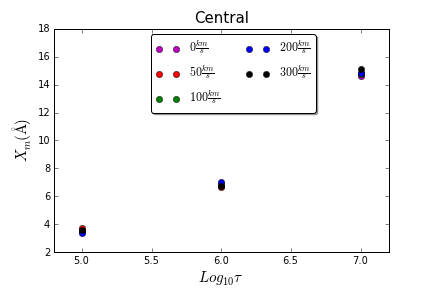
\includegraphics[width=0.45\textwidth]{maximumvsODDifSpeedsCentral.png}
%    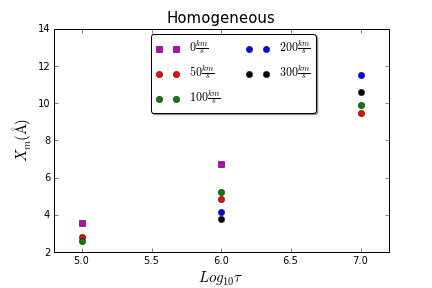
\includegraphics[width=0.45\textwidth]{maximumvsODDifSpeedsHOM.png}
%  \label{fig:maximavsOD}\caption{Position of the maxima in the
%    outgoing spectra for differents Optical Depths, (up)Central
%    Distriution, (Down) Homogeneous Distribution.} 
%\end{figure}

The second feature in the line that we use to quantify the effect of
rotation is the position of the line maxima. These provide information
on the wavelength of the majority of the outgoing photons after
they interact with the neutral hydrogen atoms in the gas cloud. If
most of the photon escapes with a low number of scattering, its
outgoing frequency will be close to its initial frequency, that is in
the center of the line. On the contrary if the number of scatterings
is large for the average photon, its outgoing frequency will be far
from the line center. Such reasoning can be made more quantitative to
understand the dependence of the peak maxima as a function of the
hydrogen optical depth in the cloud [citation needed].


In Figure ~\ref{fig:maximavsvelocity} we present the position
of the maxima as a function of $V_{\rm max}$. For the photons emitted
in the line center we do not find any variation in the position of the
maxima in the range of explored parameter space. However in the
homogeneous case we can see how the maxima goes to $x_{m}=0$, meaning
that the double peak is converted into a single peak.

This transition to a single peak line occurs for the systems where it
becomes easiear for a bulk of the photons to escape with the lowest
number of scatterings possible. This can explain how the single peak
stage can be achieved in the homogeneous source distribution where
there is fraction of the photons inside a photosphere region with
$\tau_{H}\sim 1$ which allows them to escape within one
scatter. Increasing the rotational velocity makes it easier for the
photons in this photosphere region to escape.

In Figure ~\ref{fig:maximavsangle} we present the position of the
maxima as a function of the viewing angle $\mu$ for all the optical
depths and rotational velocities and the two different photon
distributions [FALTA LA GRAFICA]. 


%Finally when we take into account the viewing angle Fig
%~\ref{fig:DifferentObservers} we found that $X_{m}$ does not depend on
%it, but again there is a threshold for the homogeneous distribution in
%which  the double peaked merged into a single peak but this time it is
%just the angle of viewing effect. 

%rotational velocities photons escape with
%less scatterings (fig:ref), for $v=100$\kms the majority of the photons
%still escape with scatterings (double-peaked line) but for $v=200$\kms
%the number of photons that escape with a few or any scatterings is higher
%(single-peaked line), this is one of the main effects of rotation. \\ 

% try a Nscatt plot as a function of theta
%explain the method

% explicar como se mide el ancho para algunos casos
% I dont understand this at all, hope Nscatts plot helps 
 %make comparison with Verhamme et al 



Finally we also report on the effect of the neutral Hydrogen
optical depth $\tau_{H}$ on the maxima position $x_{m}$
Figure~\ref{figure:maximavsOD}. We find that, at fixed
rotation velocity, the position of the maxima increases with optical
depth as expected from basic theoretical consideraions. We compare
our results with the expected theoretical escaling for an infinnite
slab. 




\subsection{Average Number of Scatterings}

Untill know we have focus in how rotation affect the morphology of the lyman alpha line, now we turn to study deeply the posible causes of this effects. As recombination is the main cause of the lyman alpha, it is important to study the relationship between the number of times that a photon is absorbed and re emitted hereafter scatterings with it's shift in the wavelenght. \\

As a first approach we study the number of scatterings of all the photons at different velocites and for both distributions Figure~\ref{fig:Nscatt}. For the central distribution the number of scattering does not change with $V_{max}$ , this implies that..., For the Homogeneous distribution we found that as $V_{max}$ increase the average number of scatterings decrease, it means that rotation..

In order to understand the double peack we make a histogram..   

as we think Nscatt is related with the double peacked line and maxima positions.


\begin{figure*}[ht]
    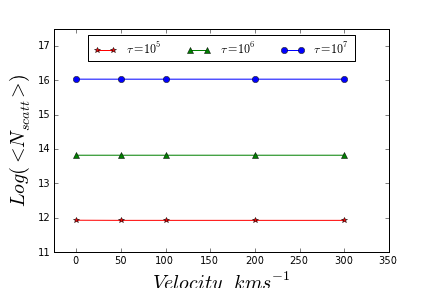
\includegraphics[width=0.45\textwidth]{NscattCentral.png}
    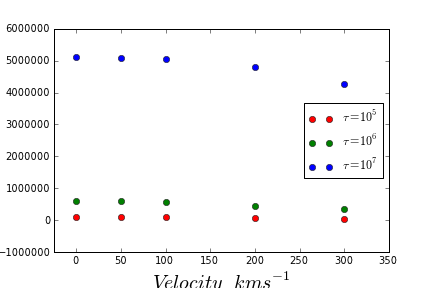
\includegraphics[width=0.45\textwidth]{NscattHOM.png}
\caption{Nscatt\label{fig:Nscatt}} 
\end{figure*}

\begin{figure*}[ht]
    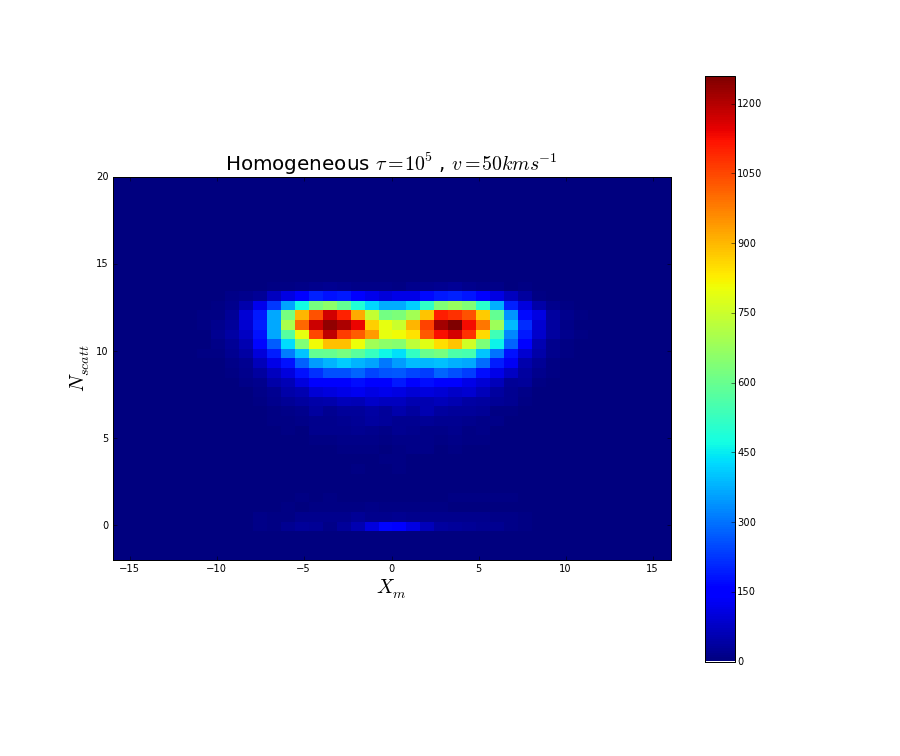
\includegraphics[width=0.45\textwidth]{2dHistogram50Central5t.png}
    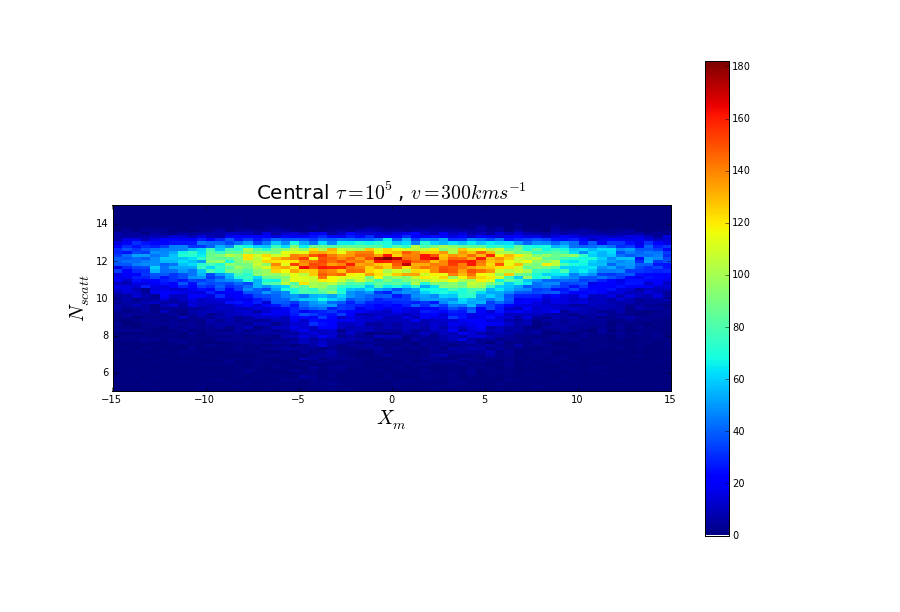
\includegraphics[width=0.45\textwidth]{2dHistogram300Central5t.png}
\caption{Nscatt\label{fig:NscattHisto}} 
\end{figure*}



\subsection{Escape Fraction}
\label{sec:EF}

We have seen in the previous section that rotation affects the number
of scatterings that ..\\

Of particular interest is to compute the escape fraction of Lyman $\alpha$ photons coming from the most distant galaxies, due to the fact that with the observed intensity of the lyman alpha line quantities as the LF and SFR can be derived (put some references). \\

Previous studies have shown the correlation of the Escape fraction with galctic mass (Lauren 2009 et al, Dayal et al 2010) abundacies and the kinematics of dust. In order to study pure rotational effects in the escape fraction we fixed the dust abundance $\tau_{A}=0.01$ and the galaxy mass. We compute the escape fraction for the models described in Table \ref{table:models}.\\

For a realistic model we also take into account the viewing angle, first we fixed the viewing angle at $\theta = 0$  Fig. and then we fixed the velocity in order to see the escape fraction correlation with the viewing angle. Therefore we define the escape fraction as:\\ 

\begin{equation}
F_{e}=\dfrac{\Sigma_{NI} \vec{k}\cdot \vec{o}}{\Sigma_{NF}\vec{k}\cdot \vec{o}}
\end{equation}

Where NI is the initial number of photons and NF is the final,
$\vec{k}$ is the rotation axis direction and $\vec{o}$ the observer
direction. With this definition we compute the escape fraction for all
of our models, the results are shown in Fig \ref{figure:escape}\\  
 
\begin{figure*}
  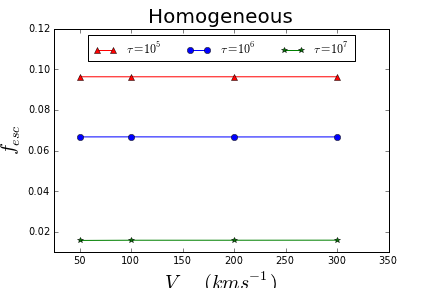
\includegraphics[width=0.45\textwidth]{FECENTRAL.png}
  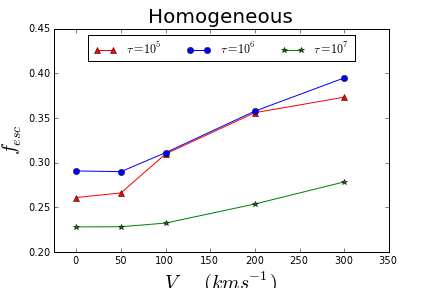
\includegraphics[width=0.45\textwidth]{FEHOMOGENEOUS.png}
   \label{figure:efvsv}\caption{Escape fraction for all the models. Left
    panels show the central distribution, while right panels show the
    homogeneous distribution} 
\end{figure*}

In Figure \ref{figure:efvsv} we found that in the central distribution the escape fraction does not change with velocity while it
does in the optical depth. On the other hand for the homogeneous distribution
we found that for higher velocities photons escape easily. The
difference between this two results relly in the fact that in the
homogeneous distribution photons are emitted closer to the escape
surface and this makes this configuration more sensitive to
rotation while in the central configuration the escape fraction depends mainly in the amount of gas rather than in rotation.    

\begin{figure*}
  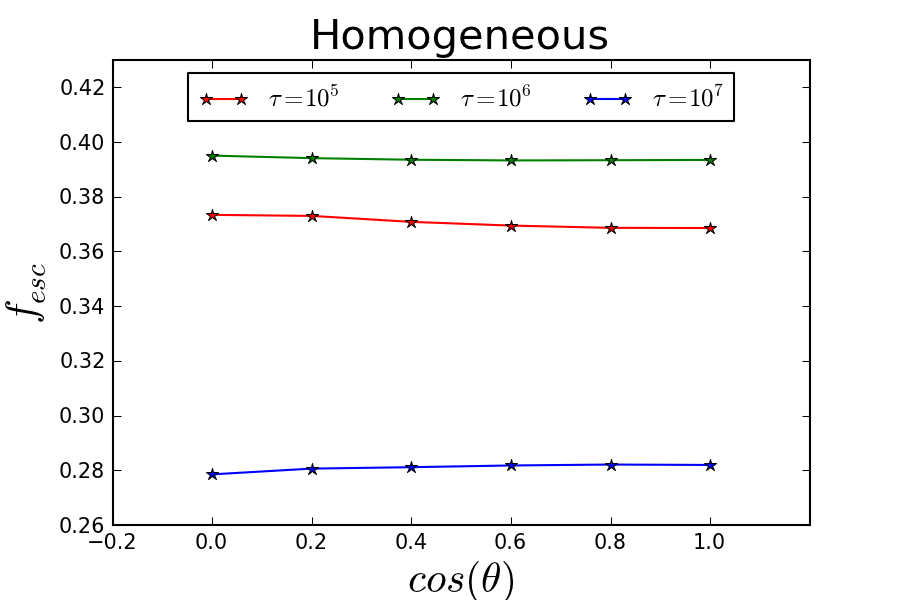
\includegraphics[width=0.45\textwidth]{FEHomogeneousvsThetaL.png}
 \label{figure:efvstheta}\caption{Escape fraction dependency with the viewing angle in the homogeneous configuration.} 
\end{figure*}

\subsection{Integrated flux}


\section{Discussion}
\label{sec:discussion}

\section{Observational implications}
% taking into account equivalent widths results with narrow band filters we can make a criterium in order to select wich galaxie could be seen in actual observations.

... The results derived in this paper have consequences on the
interpreation of galaxy observations in the Lyman alpha line.

\section{Conclusions}

\section*{Acknowledgements}

\section*{Appendix A: Tables}


\end{document}




% fix this table is too big
%\begin{table*}
%\begin{center}
%\begin{tabular}{cc}\hline
%Model & Fit\\
%Central, $\tau=10^5, V=200$\kms &$FWHM(\mu)=-149877+84509\mu-17864\mu^{2}-1677\mu^{3}-59\mu^{4}$\\
%Central, $\tau=10^6, V=200$\kms &$FWHM(\mu)=-32264+9644\mu-1080\mu^{2}+53.8\mu^{3}-\mu^{4}$\\
%Central, $\tau=10^7, V=200$\kms & $FWHM(\mu)=-1791+359\mu-27\mu^{2}+0.9\mu^{3}+0.011\mu^{4}$\\
%Hom, $\tau=10^5, V=200$\kms & $FWHM(\mu)=-51882.9+12932.5\mu-54.58\mu^{2}-187.22\mu^{3}+11.66\mu^{4}$ \\
%Hom, $\tau=10^6, V=200$\kms & $FWHM(\mu)=-7154649+2413478\mu-305268.4\mu^{2}+17158.92\mu^{3}-361.64\mu^{4}$ \\
%Hom, $\tau=10^7, V=200$\kms & $FWHM(\mu)=-51074+9912\mu-721\mu^{2}+23.29\mu^{3}-0.28\mu^{4}$ \\
%\hline
%\end{tabular}
%\caption{Fits for EW models} 
%\label{table:fits}
%\end{center}
%\end{table*}


\begin{table}
\begin{center}
\begin{tabular}{ccc}\hline          
Velocity (Km/s) & Maximum 1 position & Maximum 2 position \\ \hline
50 & -16.2695 & 16.23705 \\ 
100 & -15.66496 & 15.33504 \\ 
200 & -16.93149 & 14.56851 \\ 
300 & -13.40048 & 16.09952 \\ \hline 
\end{tabular} 
\caption{Optical Depth $\tau= 10^{7}$, Central Distribution}
\end{center}
\end{table}

\begin{table}
\begin{center}
\begin{tabular}{ccc}\hline 
Velocity (km/s) & Maximum 1 position & Maximum 2 position\\ \hline
50 & -7.46286 & 6.53714 \\ 
100 & -7.53357 & 6.96643 \\ 
200 & -8.17453 & 7.32547 \\ 
300 & -6.81487 & 6.18513 \\ \hline 
\end{tabular} 
\end{center}
\caption{Optical Depth $\tau = 10^{6}$, Central Distribution}
\end{table}

\begin{table}
\begin{center}
\begin{tabular}{ccc}\hline 
Velocity(Km/s) & Maximum 1 position & Maximum 2 position\\ \hline
50 & -4.33708 & 3.66292 \\ 
100 & -4.27326 & 3.72674 \\ 
200 & -3.7737 & 3.7263   \\ 
300 & -3.84903 & 4.15097 \\ \hline 
\end{tabular}
\caption{Optical Depth $\tau=10^{5}$, Central distribution} 
\end{center}
\end{table}

Line width\\

\begin{table}
\begin{center}
\begin{tabular}{ccc}\hline 
Velocity(Km/s) & FWHM & $\theta$\\ \hline 
50 & 12.62 & $0^{o}$ \\ 
50 & 12.72 & $45^{o}$ \\ 
50 & 12.93 & $90^{o}$ \\ 
100 & 14.07 & $0^{o}$ \\ 
100 & 14.48 & $45^{o}$ \\ 
100 & 15.00 & $90^{o}$ \\ 
200 & 16.90 & $0^{o}$  \\ 
200 & 18.51 & $45^{o}$ \\ 
200 & 21.24 & $90^{o}$ \\ 
300 & $24.69^{*}$ & $0^{o}$ \\ 
300 & $25.79^{*}$ & $45^{o}$  \\ 
300 & $27.73^{*}$ & $90^{o}$ \\ \hline
\end{tabular}
\caption{Lines Widhts for a Central Distribution and $\tau=10^{7}$} 
\end{center}
\end{table}


Escape fraction\\

\begin{table}[H]
\begin{center}
\begin{tabular}{ccccc}\hline 
Model & Velocity (km/s) & $\theta$ & Dust $\sum (s)$& $\sum (s)$\\ \hline 
Homogeneous & 50 & $0^{o}$& 13293.06 &49939.53\\ 
Homogeneous & 50 & $45^{o}$& 13291.04 &50001.59\\ 
Homogeneous & 50 & $90^{o}$ & 13348.76 &49922.73\\ 
Homogeneous & 100 & $0^{o}$ & 15527.69 &50114.11\\ 
Homogeneous & 100 & $45^{o}$ & 15511.56 &49967.17\\ 
Homogeneous & 100 & $90^{o}$ & 15401.71 & 49833.65\\ 
Homogeneous & 200 & $0^{o}$  & 17830.85 & 50078.69\\ 
Homogeneous & 200 & $45^{o}$ & 17932.87 & 50064.42\\ 
Homogeneous & 200 & $90^{o}$ & 17830.85  & 49931.748\\ 
Homogeneous & 300 & $ 0^{o}$ & 18687.33 & 50048.33 \\ 
Homogeneous & 300 & $45^{o}$ & 18572.12& 49922.67\\ 
Homogeneous & 300 & $90^{o}$ & 18421.79 & 49979.37\\ \hline
\end{tabular}
\caption{Escape fraction for a Homogeneous Distribution and optical depth $10^{5}$.} 
\end{center}
\end{table}


\begin{table}
\begin{center}
\begin{tabular}{ccccc} \hline 
Model & Velocity (km/s) & $\theta$ & Dust $\sum (s)$& $\sum (s)$ \\  \hline 
Central & 50 & $0^{o}$ & 4809.881 & 49917.069 \\ 
Central & 50 & $45^{o}$ & 4829.21 & 49811.79 \\ 
Central & 50 & $90^{o}$ & 4845.108 & 49853.039\\ 
Central & 100 & $0^{o}$ & 4809.665 & 49921.30 \\  
Central & 100 & $45^{o}$ & 4828.65 & 49820.13 \\ 
Central & 100 & $90^{o}$ & 4846.45 & 49854.0 \\ 
Central & 200 & $0^{o}$  & 4809.63 & 49917.64 \\ 
Central & 200 & $45^{o}$ & 4829.25 & 49818.49 \\ 
Central & 200 & $90^{o}$ & 4844.89 & 49856.66 \\ 
Central & 300 & $ 0^{o}$ & 4810.56 & 49922.98\\ 
Central & 300 & $45^{o}$ & 4831.16 & 49823.33\\ 
Central & 300 & $90^{o}$ & 4845.33 & 49858.48\\ \hline
\end{tabular}
\caption{Escape fraction for the central Distribution and optical depth $10^{5}$.} 
\end{center}
\end{table}


%ideas:
Keep in mind making a follow up paper on the results of Yamada et atl http://adsabs.harvard.edu/abs/2012ApJ...751...29Y on the line morphology at z=3.1. How many of these laes can be considered to have rotation features? In principle, all of then should have them. How to make the case convincing in the statistical sense?


% Bibliography
%-----------------------------------------------------------------
%\begin{thebibliography}{99}

%\bibitem{Cd94} Author, \emph{Title}, Journal/Editor, (year)

%\end{thebibliography}

